\chapter[System Description]{System Description}
\label{chap:system_description}

This chapter is about to describe the equipment used and its integration explaining how it was modeled and implemented in both hardware and software sides.

\section{System Description}
\label{sec:system_description}

\subsection{Instrumentation}
\label{subsec:instrumentation}

The main instruments used for this project are listed above:

\begin{enumerate}[a)]

  \item High Voltage Power Supply (HVPS)
  
     - brand: FUG
    
     - model: HCP35-20kV
    
    HVPS provides the electrical potential to the liquid, which can be applied by connecting the HVPS directly to the liquid feeding capillary or needle to a grounded electrode (usually a plate or a ring) located downstream.\cite{Monica}
    The setup has the USB serial interface for controlling and polling measurements.
    
    The software has an interface to integrate the HVPS to our routine. This interface can be found in \emph{FUG\_function.py} file where is located the functions used to control and collect data from this instrument.
    In case of future change of equipment brand a new interface must be created within this file to match another manufacturer specifications.

  \item Wireless Oscilloscope
  
     - Brand: \emph{TiePie engineering}

     - model: TiePie WifiScope WS6 DIFF
    
    The signal analysis with an oscilloscope using WiFi technology allows an in-depth case study of the electric current signal.
    The current is measured via a TiePie WifiScope WS6 from TiePie engineering that is a battery powered oscilloscope capable of transmitting data via a WiFi connection allowing it to be placed in the high voltage or ground path.
    
    Wireless communication allows us to make measurements disconnected to an external power supply, which gives us more safety when using high voltage potential references and also reduce the signal noise collected from external power lines.
    The current is routed directly via the input, hence the oscilloscope measures the voltage dropped via its input resistance (which can be switched between 1 or 2 M%Ω).
    TiePie WifiScope WS6 has a resolution of up to 16 bit at a minimal input range of 200 mV, sufficient to measure currents down to 1 nA.

    The interface with the software was made using the TiePie Library\cite{TiePieLib} and can be found in \emph{configuration\_tiepie.py}. Note that is also important to have the \emph{printinfo.py} file in the project folder in order to work.

  \item Humidity and Temperature sensor
  
  The stability of the system is aftected by many physical effects. Evidently having the more parameters analysed favours the system control.
  The surface tension force is dependant of the liquid-gas interface on the meniscus. Hence, the gas around it must be constantly the same and so its humidity.
  Also, temperature is a variable that interfere in many phenomenas in the system. Specially the liquid properties such as viscosity.

  For that, a standart microcontroler development board (\emph{Arduino Uno}) with a temperature and humidity sensor (DHT11) was configured to add that data in real time in the routine.
  The Arduino code can be found in the \emph{/peripherals} folder.
  

  \item High Speed Camera 
  
  - Brand: \emph{Photron}

  - model: Photron fastcam mini


  
  \item Syringe pump
  
  - Brand: \emph{Master dual}

  - model: WPI AL-1000

  The pump integration in the automation algorithm bring us a new controllable variable, the Flowrate. Now we can control the spraying mode with the
    two main variables that afect the system. 
    It will bring more complexity for the system since now we are dealing with multivariable control.
    Controlling also the flowrate gives to this project a new dimension in the system giving us freedom to explore the flowrate properties.
    % Our control model is now a MISO \footcite{MISO: Multiple Inputs Single Output} system. The crossover (couple) between the controlled variables will be evaluated in further reports.

    About the pump interface. As I could not find a good ready-to-use library for this pump I developed an simple and intuitive interface to be our software routine.
    The communication protocol used is RS-232. In the software routine the communication used is python serial interface. The pump commands list were found in the user manual.

  
  Also, the supply of constant pressure can also 
    \cite{prunet}
  The supply at constant pressure sometimes favours the stability of the spray. However, the flow rate depends on the applied pressure and pressure losses between the tank and the end of the capillary, which themselves are dependent on the liquid chosen and on its temperature. This volume flow rate may also depend on the applied voltage, since the electrostatic pressure on the meniscus produces a suction effect.


  \end{enumerate}



\subsection{Setup Organization}
\label{subsec:setup_organization}


\begin{figure}[H]
  \centering
  \resizebox{150mm}{!}{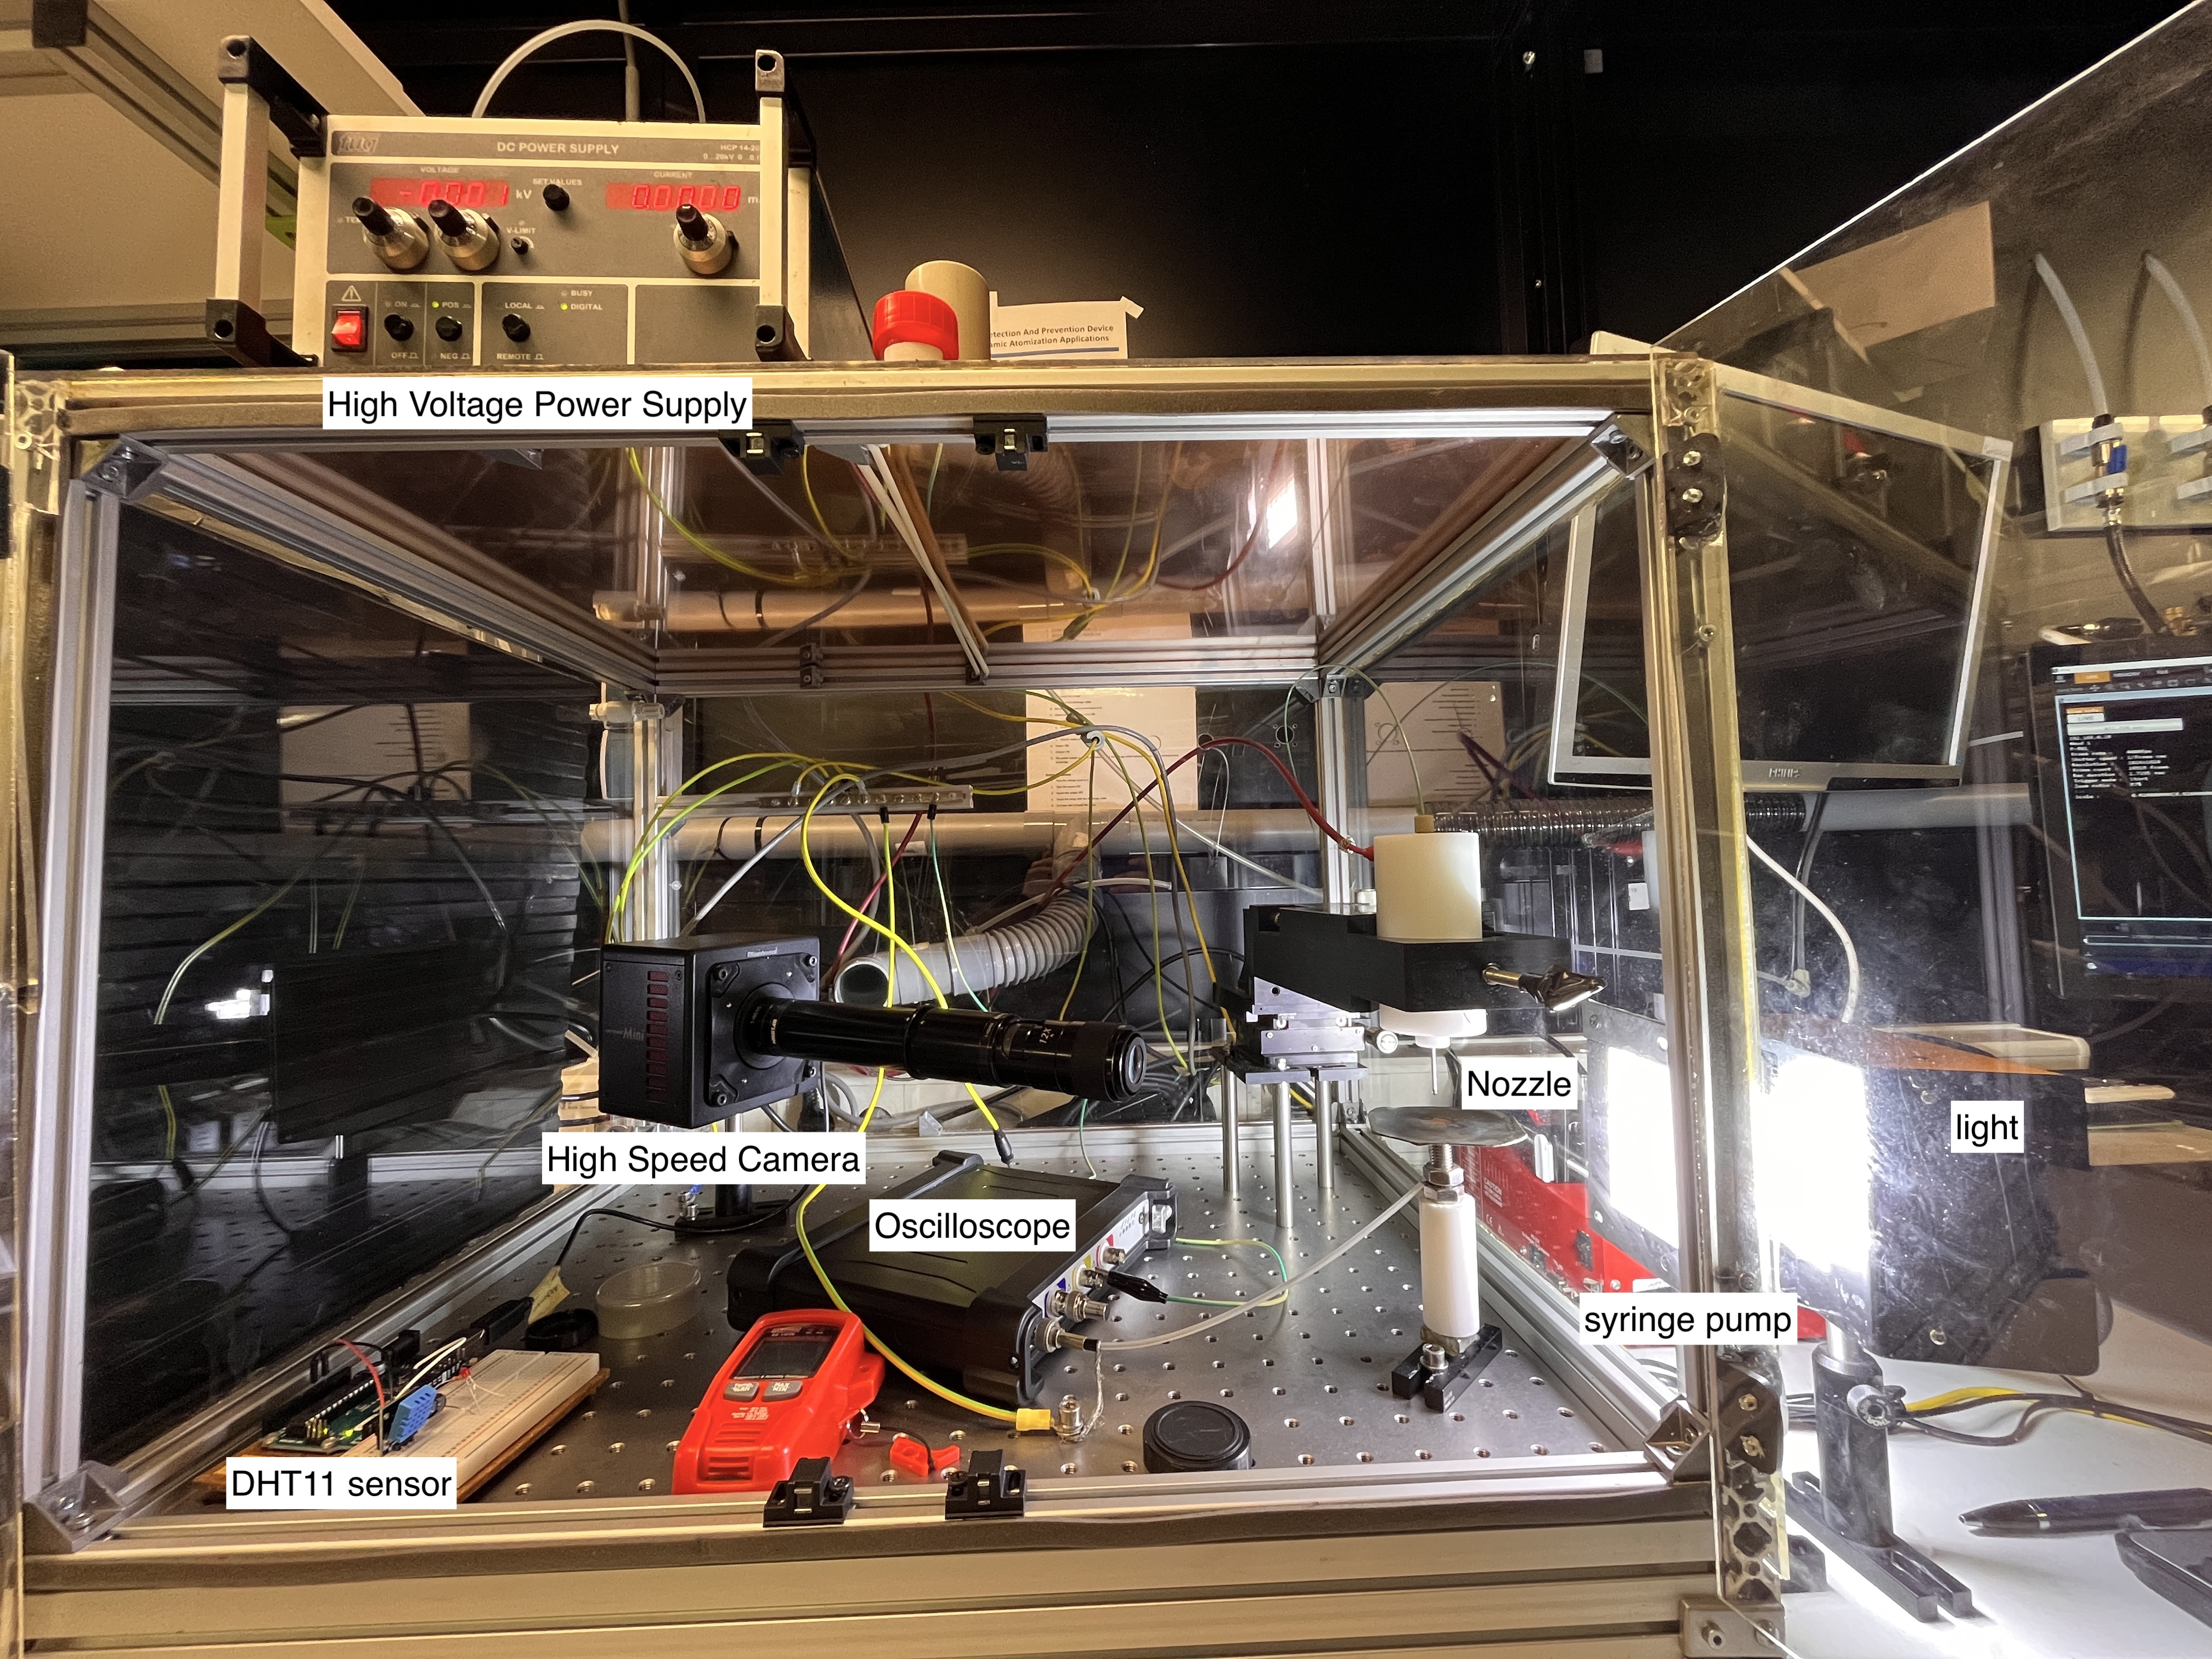
\includegraphics{Figuras/setup_pic.jpg}}
  \caption{EHDA automation system setup}
  \label{fig:setup_pic}
\end{figure}


The peripherals automation routine was already developed by another student. In order to continue the research I took some time to understand the physical concept behind EHDA experiments and the project knowledge.
I made upgrades in the routine to include the high speed camera with a hardware triggering routine using an arduino microcontroler. This will be usefull to validate the further classification of the spray dynamics.

% ilustramos o processo com a Figura \ref{fig:setup}. 

\begin{figure}[H]
  \centering
  \resizebox{150mm}{!}{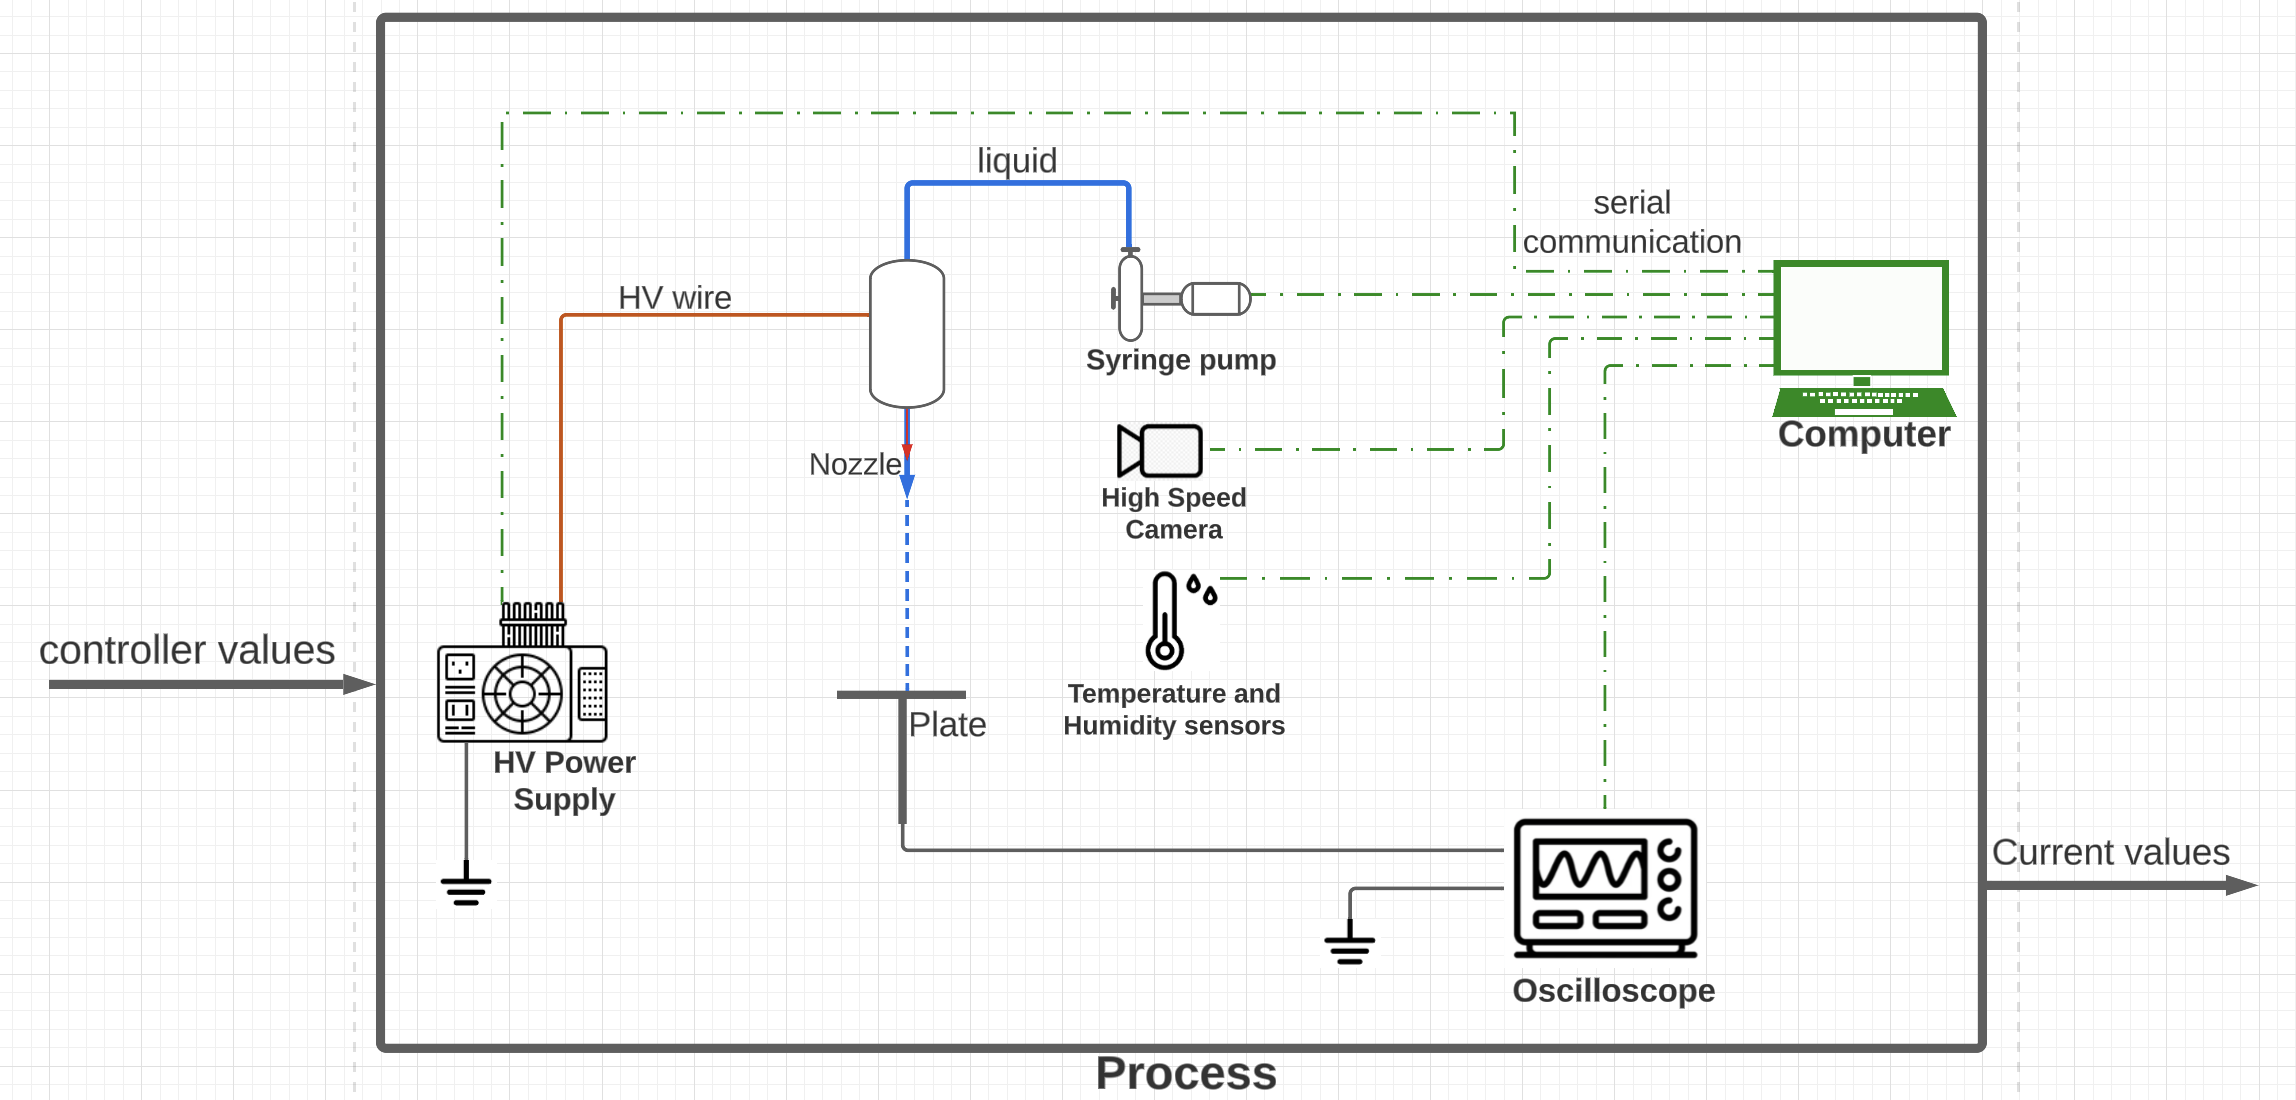
\includegraphics{Figuras/new_system_setup.png}}
  \caption{EHDA automation system setup}
  \label{fig:setup}
\end{figure}


\subsection{Setup Validation}
\label{subsec:setup_validation}

Initial tests were made to verify the setup assembly and the automation routine integration. In this step I could unterstand in practise how electrospray works.
I noticed that we need a large set of variables in the range to produce the desired dynamics of electrospray, which most of the time is cone-jet mode.
 Those variables can be the liquid properties such as surface tension, dielectric constant, viscosity, density, electrical conductivity and vacuum permitivity. 
 And also physical variables such as flowrate, system impedance, system temperature, system humidity, nozzle to plate distance, nozzle dimensions and applied voltage.


 About the setup,integrate was changed the liquid, nozzle diameter and distance to the plate in order to
make the experiment the most stable and easy to reach cone-jet mode as possible. For example, while doing experiments we discovered that the frequency of the pump machine internal motors was creating an interference in the flowrate. Therefore compromising the stabilization in cone jet mode. A solution for that was to increasethe flowrate wich smooths this pumping noise. For that was also necessary to increase the nozzle diameter to balance with all other variables from the experiment.


    
    \begin{figure}[H]
        \centering
        \resizebox{150mm}{!}{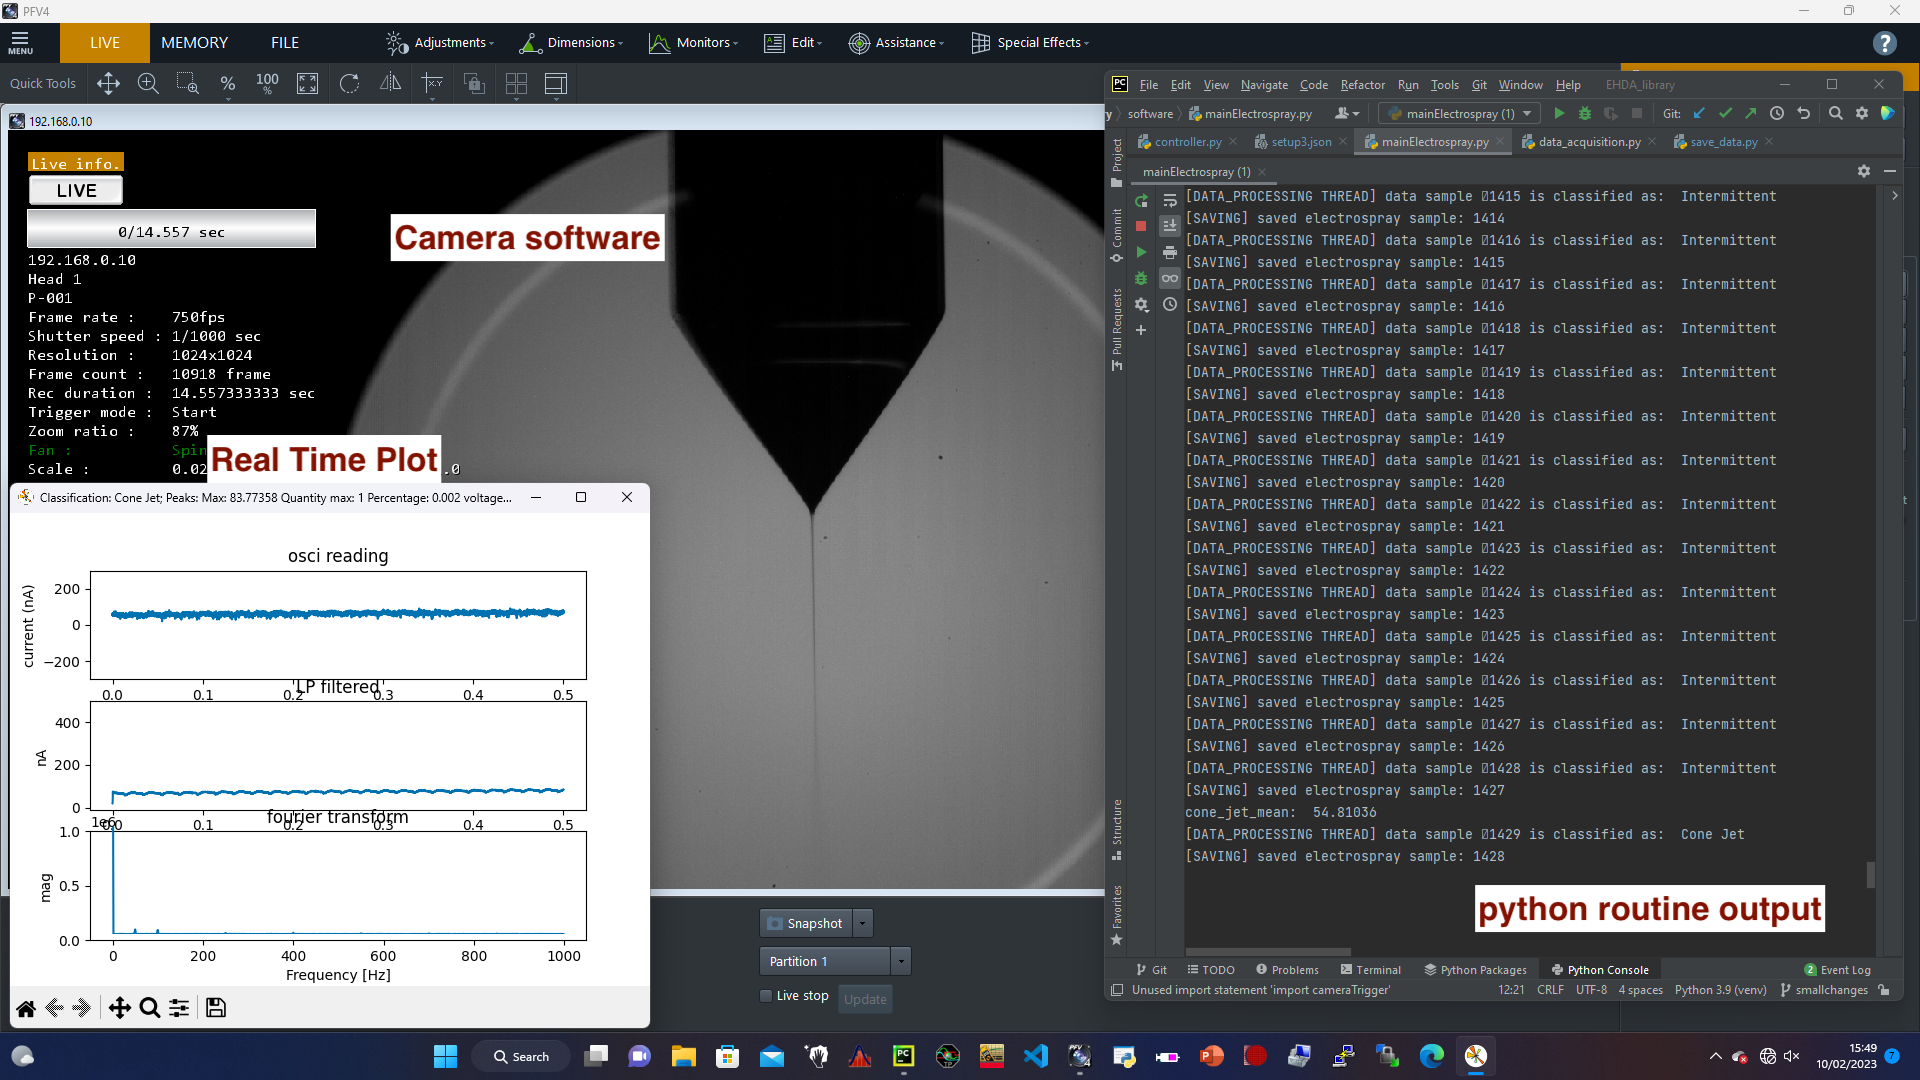
\includegraphics{Figuras/report4/experiment_print1.png}}
        \caption{EHDA automation system setup}
        \label{fig:metodology_example1}
    \end{figure}

\section{System Model}
\label{sec:control_model}

ilustramos o processo com a Figura \ref{fig:control_model_fig}. 

\begin{figure}[H]
  \centering
  \resizebox{150mm}{!}{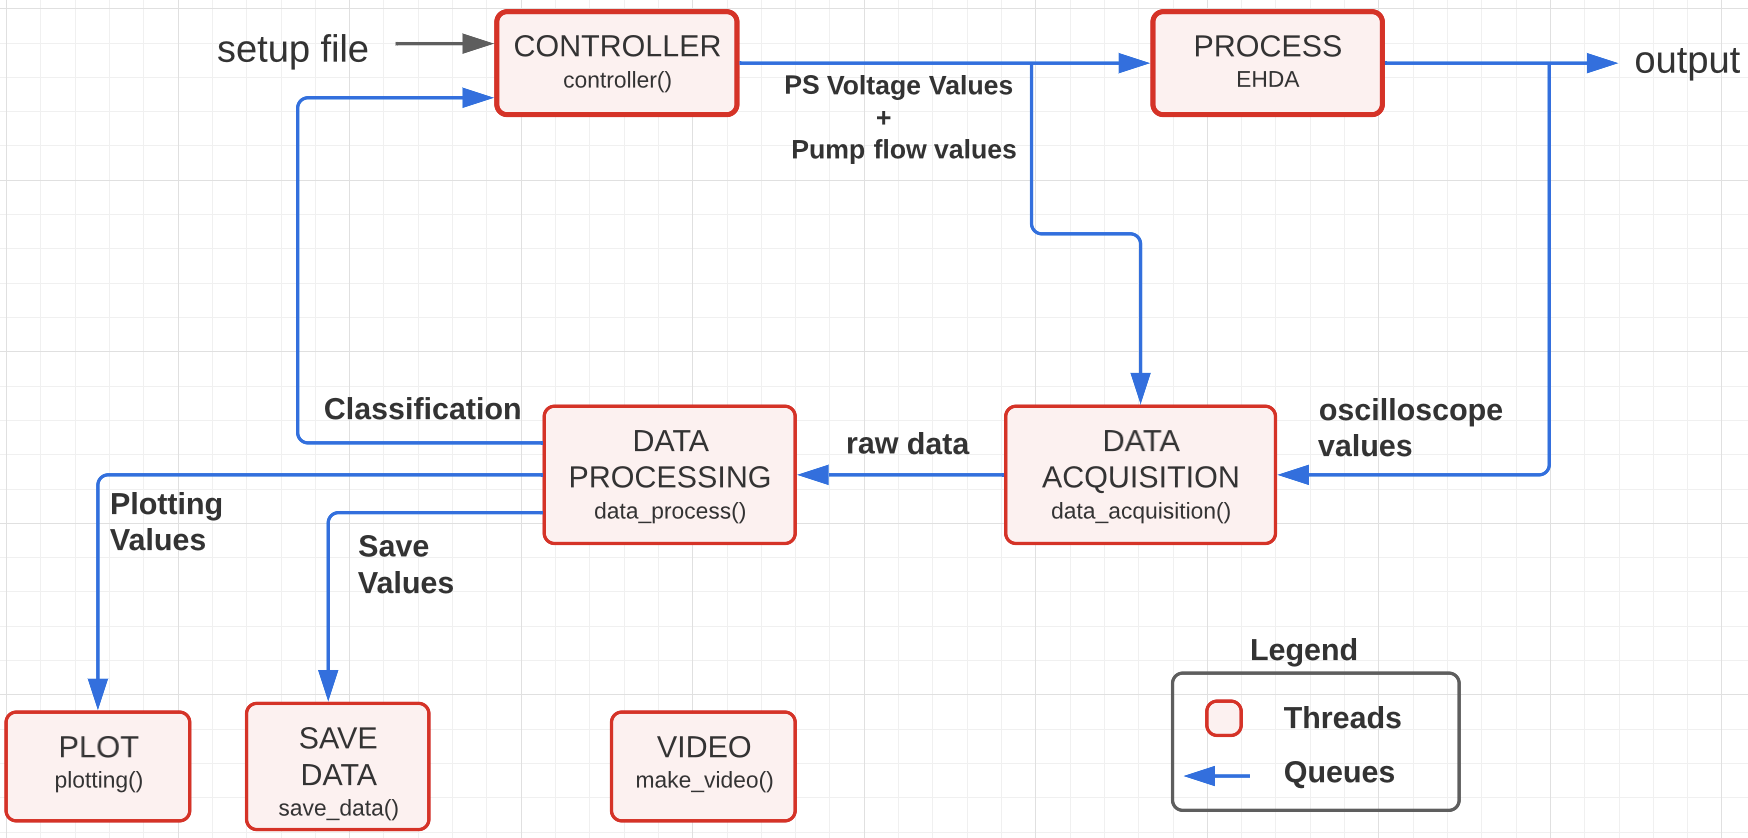
\includegraphics{Figuras/control_loop.png}}
  \caption{EHDA automation system setup}
  \label{fig:control_model_fig}
\end{figure}

\subsection{Threading and Queues}
\label{subsec:concurrency}

    In order to implement this system model to the software and explore parallel processing each system in the
    model was developed as a separate Thread.
    For cuncurrency on flux of data between threads was used queues structures.
    A queue is an abstract data type that holds an ordered, linear sequence of items. You can describe it as a first in, first out (FIFO) structure.

    
    \subsection{Controller Thread}

        It is responsible of sending the power supply set voltage values and the syringe pump the flow rate set values according to the sequence selected.
        Also responsible of sending the finish event command that end the routine and trigger the threads to close their routines.
        As input we have the setup config file and the \emph{feedback\_queue}. As output we have the values in the emph{controller\_output\_queue()}.

    \subsection{Data Acquisition Thread}
    \label{subsec:data_aquisition}

        It is responsible for reading the current data from the oscilloscope, humidity and temperature data from the DHT11 sensor, voltage from the powersupply, flowrate from the pump and concatenate into one sample data.
        As output we have the values in the emph{data\_queue()}.

    \subsection{Data Processing Thread}

        It is responsible for calculating the statistical values from the raw data and classify it in the respective spray mode for that sample.
        As output we have the values in the emph{save\_data\_queue()}, emph{plotting\_queue()} and emph{feedback\_queue()}.
    
        \subsection{Save Data Thread}

        After the processing the data is saved in real time in a json file using \emph{jsonstreams} library to save one sample structure at a time.

        With the new streamming model of saving a new structure of the collected data were created.
        Instead of having all data measurements values and after all data processing values we now are saving for each sample the measurements and processing values.
        The structure of the 
    
        \begin{figure}[H]
            \center
            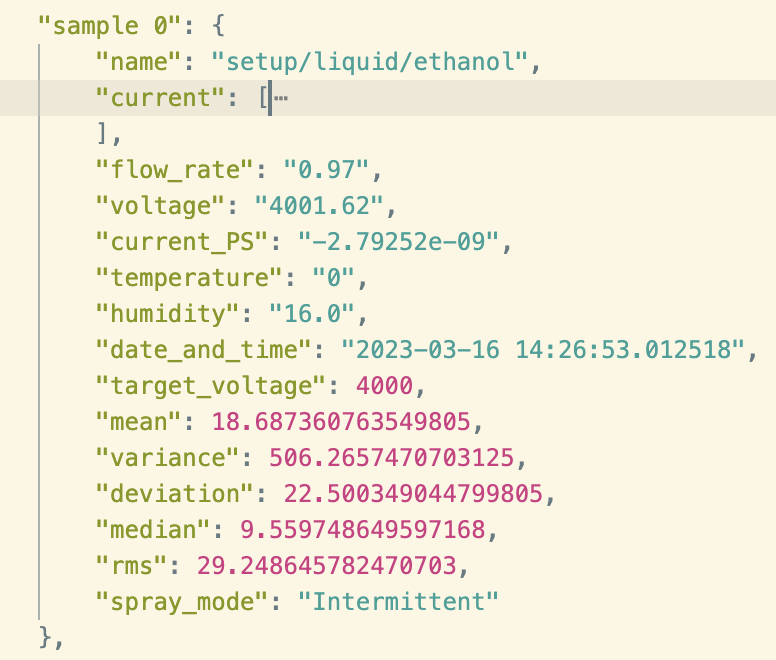
\includegraphics[width=10cm]{Figuras/19:03/new_sample.png}
            \caption{Output data json structure}
        \end{figure}
    
        To work with this data I'm using pandas Dataframe.
        With the command:
        
        pandas.read\_json('PATH', orient='index').
    
        The json file is good to store the data and to read the file. But as it is getting a lot of data working with pandas Dataframe is being way faster. Also saving the dataframe in a compressed
        type of file called feather is much faster to work with the data.
    
    \subsection{Video Thread}

        Normally deactivated, that thread is responsible for triggering the camera in case we want to save a video of that sample.
    
    \subsection{Plot}

        The only running function that is not a thread because of the plotting library \emph{matplotlib} incompatibilites of running outside of the main function. 
        It is responsible of plotting in real time the current sample acquired and it respective fast fourier transform to evaluate the sample frequency spectrum.
    
    
    - plotting data queue

\clearpage
